\documentclass[journal,12pt,a4paper,compsoc,onecolumn]{IEEEtran}
\IEEEoverridecommandlockouts
\usepackage{cite}
\usepackage[colorlinks,linkcolor=black,anchorcolor=blue,citecolor=red]{hyperref}
\usepackage{amsmath,amssymb,amsfonts}
\usepackage{algorithmic}
\usepackage{graphicx}
\usepackage{textcomp}
\usepackage{xcolor}
\usepackage{amssymb}
\usepackage{subcaption}
\usepackage{threeparttable}
\usepackage{pdfpages}
\usepackage{hyperref}
\def\BibTeX{{\rm B\kern-.05em{\sc i\kern-.025em b}\kern-.08em
    T\kern-.1667em\lower.7ex\hbox{E}\kern-.125emX}}
\newcommand{\upcite}[1]{\textsuperscript{\cite{#1}}}
\pagenumbering{arabic}
\def\IEEEkeywordsname{Keywords}
\def\figurename{Figure}
\begin{document}

\title{LittleGAN: Conditional Facial Image Generation and Adjustment}
\author{Yongxiang Meng, Wenyan Chen\\Guangzhou No.6 Middle School, China}
\hypersetup{
	pdftitle=LittleGAN: Conditional Facial Image Generation and Adjustment,
	pdfauthor=Yongxiang Meng\, Wenyan Chen
}


\includepdf[noautoscale]{attach/info-en.pdf}
\includepdf[noautoscale]{attach/info.pdf}


\maketitle
\begin{abstract}

In daily life, it is often necessary to pass portrait information, such as obtaining images from eyewitness in public security.
However, traditional method has some disadvantages and existing machine learning model's use-cost is too high.
Through a large scale of experiments, we propose a single multi-task model for conditional facial image generation and adjustment.
The proposed model based on DCGAN, inspired by pix2pix and PGGAN.
Major improvements are as follows.
We share parameters between GAN and Adjustor,
    reducing the size of the model and use-cost compared to two individual models.
We adjust images in the image space,
    reducing the loss of original image information.
We propose a method of partition training,
    making deep neural network easier to train.
It is validated that the model can validly generate plausible facial images from attributes and be adjusted by attributes.
Results also suggest that the use-cost of LittleGAN has declined.
Compared to DCGAN and pix2pix, it can be more effectively applied to the actual production activity.

    \begin{IEEEkeywords}
        Facial Image Generation, Facial Image Adjustment, Generative Adversarial Networks, Machine Learning
    \end{IEEEkeywords}

\end{abstract}
\newpage
\tableofcontents
\newpage
\section{Introduction}

In recent years, machine learning has gone deeply in the society.
Facial image generation and facial image adjustment are one of the directions.
As an important characteristic, face makes a difference in the interpersonal activities.
Combined with the technology of face identification, facial image generation can be used to define identity.
The technology mainly applies to identity authentication, used to chase the target, which is a vital auxiliary method to combat criminal activities.
When it comes to social activities, it can also be utilized to the identification of intelligent interaction scene.
For example, the safety detection at the school gate and the check point of the company.

Nowadays, under the circumstances of the disability to get the exact figure,
    public safety agency mainly adopt the following method.
According to the description of eyewitness, corporate with the painter to get the rough facial image,
    search for the figure in the existent image data base and confirm the identity of the figure.
We assume that the method has large shortcomings.
First, the subjective consciousness of the painter will affect the generation of the portrait.
    The second is that the painter's painting quality is higher and the cost is higher,
    and the third is that the speed of image generation is higher in certain occasions.
The method of tracking and positioning according to the photo of the target person may also cause the face of the target person to be inaccurate due to the problem of poor photographing angle or the long time of taking photos.
The research on adjusting the attribute of the face image is used to solve this problem.
This research has certain practical significance for the fields that need the images of accurate target figures more quickly,
    such as accurate positioning targets in criminal investigation and speeding up the speed of solving crimes.
\section{Related Work}


\subsection{Generative Adversarial Network}
Generative Adversarial Networks (GAN) consists of two networks, the generator and discriminator.
The training process is a competition between the generator and discriminator.
The discriminator is trained to separate data from the generator from the training set,
    while the generator changes itself to let discriminator believe its output coming from real data.
In that way, the generator achieves the goal of imitating the training dataset.

Our baseline model, DCGAN, is a type of GAN that uses convolutions to replace fully connected layers for a more stable training process.


\subsection{Image Generation}

Text-to-Image\upcite{text2img} is a method based on DCGAN\upcite{dcgan} for generating images from text description.
They combine embeded description with noise to generate images through convolution.
InfoGAN\upcite{infogan} is able to extract attributes from images, enabling conditional generation of images through unsupervised learning.
% BEGAN\upcite{began} use a variational auto-encoder as the discriminator.
% It provides a hyperparameter to adjust the balance between image variety and quality while maintaining training stability.
PGGAN\upcite{pggan} first trains on low-resolution facial image, then gradually adds network layers for training to improve the resolution of output images and the stability of the network.

\subsection{Image Translation}
Image translation works with images as both inputs and outputs.
Pix2pix\upcite{pix2pix} uses U-Net network, L1 Loss.
Theirs generator contains a U-Net combining an encoder with a decoder,
    reducing pressure on each network layer and retaining more original image information.
Theirs discriminator uses L1 Loss to globally constrain images.
In that case, pix2pix\upcite{pix2pix} can generate images better.
CycleGAN\upcite{cyclegan} uses two generators and two discriminators to train separately achieving image conversion between two attribute domains.

Whether it is pix2pix\upcite{pix2pix} or CycleGAN\upcite{cyclegan},
    although they can convert image attributes better,
    it is limited to two definite domains.
If it is required to convert multiple attributes, multiple models are needed.
In that case, model size and computational load are too large to meet actual needs.

\subsection{Facial Image Adjustment}
StarGAN\upcite{stargan} train across datasets so that the model can learn attributes and features from more datasets.
It can generate images by specifying more attributes.
AttGAN\upcite{attgan} extracts the attributes and noise of images,
    change attributes and combine noise to generate images.
It realizes adjustment of facial images.
But the process of extracting attributes and noise will cause information loss.
So, some features of original images will be lost in the adjusted images.
TPGAN\upcite{tpgan} uses a variety of Loss to achieve the multi-angle transformation of facial images.
Main method of the research is to build a facial outline and then add more details.



\vspace{3ex}

From the above analysis of current situation,
    we can learn that current facial image generation and adjustment in the face research are generally separate.
Also, different models are required to be used.
The conversion of model is likely to cause certain information loss.
Therefore, we hope to use one model to complete two tasks of facial image generation and adjustment.
In this way, not only network parameters can be shared,
    but also the time and use-cost can be reduced.
During the generation and adjustment process, attribute parameters are unified,
    avoiding extra consumption caused by the conversion between different models.
\section{Goal and Highlight}

\subsection{Research Goal}
Provide a
facial image generation and adjustment model
with good performance
and low use-cost

\begin{itemize}
\item
Propose a machine learning technology network that addresses the needs of facial image generation and adjustment for real-time applications.
It can replace traditional methods that have certain defects, such as poor real-time performance and time consuming.
\item
Combine current demand and most up-to-date work to improve the model and training methods,
    and to reduce the size and use-cost of resulting models.
\item
Apply new methods to adjust images so as to reduce information loss of original image.
\end{itemize}
\subsection{Research Highlight}
\begin{itemize}
\item
We propose a single model to perform two tasks: conditional generation and adjustment.
Also, the model has a good performance.
\item
We effectively reduce model size and cut down computational load in training and runtime by sharing parameters.
We achieve the purpose of reducing the use-cost of training, deployment and running.
\item
We propose and apply partition training method.
It alleviates the problem of vanishing gradients in previous layers of deep network,
    make it easier for deep neural networks to find the global minimum.

\item
We adjust facial images in the image space to reduce the information loss of original image.
\end{itemize}
\section{Process}
\subsection{Overall Roadmap}

In order to obtain a smaller model, less training and running with better performance,
we decided to make multiple models and training improvements based on DCGAN\upcite{dcgan} and improved it through multiple sets of experiment.
Figure \ref{roadmap} is the overall technical roadmap of this study.

\begin{figure}
    \begin{center}
    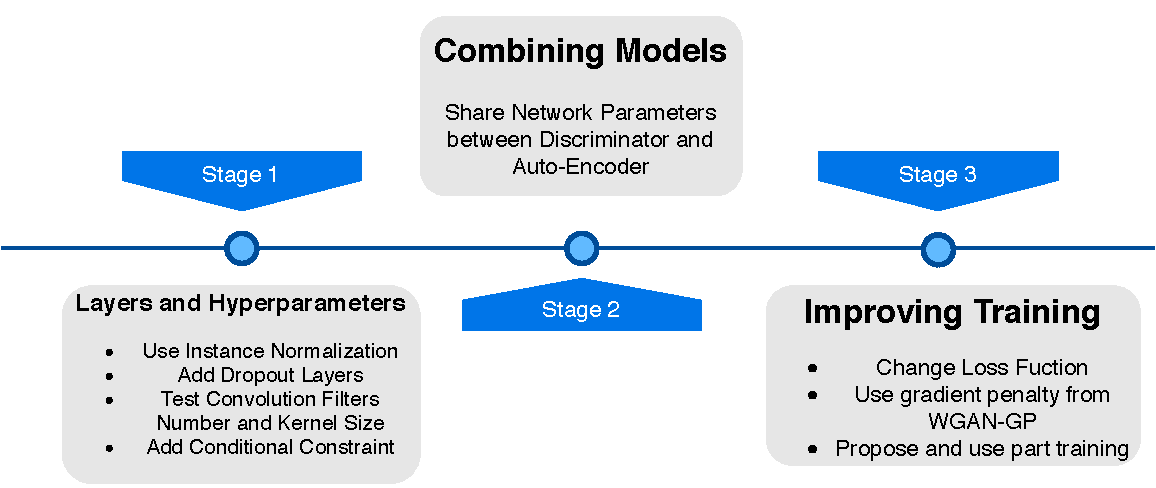
\includegraphics[width=\textwidth]{figures/roadmap.pdf}
    \caption{Overall technical Roadmap}
    \label{roadmap}
    \end{center}
\end{figure}


\subsection{Research Process}

In previous model adjustments, we conducted several comparative tests to select suitable hyperparameters.

Figure \ref{norm_bach} and Figure \ref{norm_instance} show the results of model after training 2 epochs using batch normalization and instance normalization respectively (about 5500 iterations per epoch).
It can be seen that the image quality is improved under the same training amount after using instance normalization,
    which means that the convergence speed of the model is faster.

\begin{figure}
    \begin{minipage}[t]{0.48\linewidth}
        \centering
        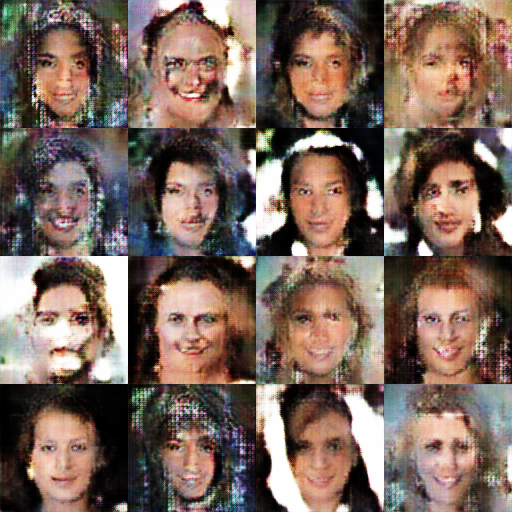
\includegraphics[width=\textwidth]{figures/result_norm_batch.png}
        \caption{Test result using Batch Normalization after training 2 epochs}
        \label{norm_bach}
    \end{minipage}
        \hfill
    \begin{minipage}[t]{0.48\linewidth}
        \centering
        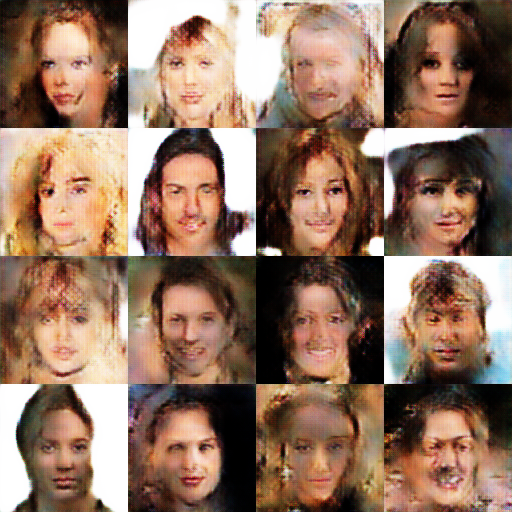
\includegraphics[width=\textwidth]{figures/result_norm_instance.png}
        \caption{Test result using Instance Normalization after training 2 epochs}
        \label{norm_instance}
    \end{minipage}
\end{figure}

In addition, we tested the effects of convolution kernel size and numbers of convolution filters on model performance and model size.
Fig.\ref{conv_filter_16}, Fig.\ref{conv_filter_24}, and Fig.\ref{conv_filter_32} are convolution filters using 16 times, 24 times, and 32 times,
    respectively and the output results are completed after training 15 epochs.
Times of convolution filters mean the start amount of convolution kernel.
It will be doubled in each next layer of decoder and encoder.
It can be seen that after the convolution filters is lowered,
    the image quality does not decrease markedly under the same training amount.
In order to reduce the size of the model to achieve the purpose of reducing use-cost,
    we finally chose a 16 times convolution filters.

\begin{figure}
    \begin{minipage}[t]{0.48\linewidth}
        \centering
        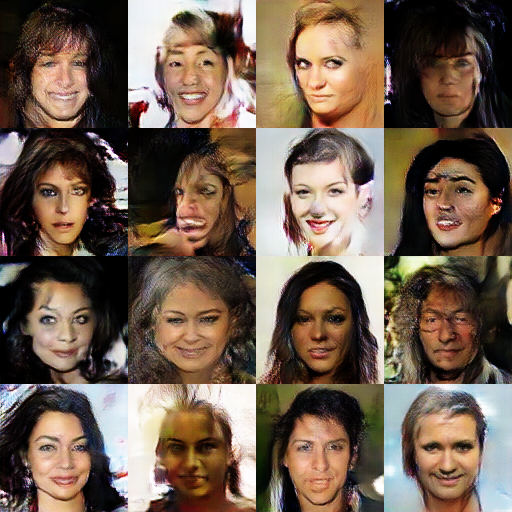
\includegraphics[width=\textwidth]{figures/result_conv_filter_16.png}
        \caption{Test result using 16x convolution filter after training 15 epochs}
        \label{conv_filter_16}
    \end{minipage}
        \hfill
    \begin{minipage}[t]{0.48\linewidth}
        \centering
        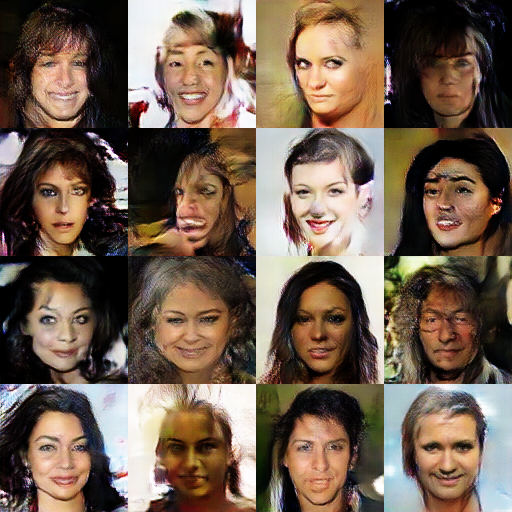
\includegraphics[width=\textwidth]{figures/result_conv_filter_24.png}
        \caption{Test result using 24x convolution filter after training 15 epochs}
        \label{conv_filter_24}
    \end{minipage}
    \begin{minipage}[t]{\linewidth}
        \centering
        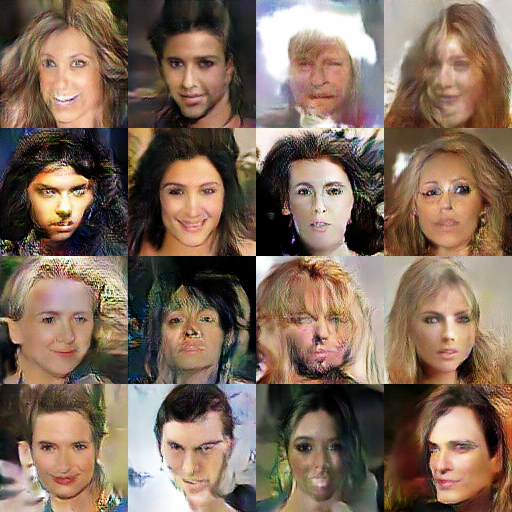
\includegraphics[width=0.48\textwidth]{figures/result_conv_filter_32.png}
        \caption{Test result using 32x convolution filter after training 15 epochs}
        \label{conv_filter_32}
    \end{minipage}
\end{figure}

Figure \ref{conv_kernel_5} and \ref{conv_kernel_3} show the results after training 4 epochs of the 5×5 and 3×3 (transposed) convolution kernel,
    respectively, under a 16 times convolution filter.
It can be seen that switching from a 5×5 convolution kernel to a 3×3 size,
    the image quality is degraded within an acceptable range, so we choose a 3×3 convolution kernel.

\begin{figure}
    \begin{minipage}[t]{0.48\linewidth}
        \centering
        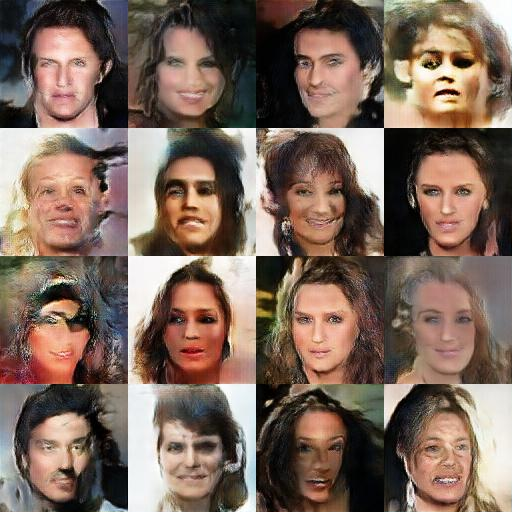
\includegraphics[width=\textwidth]{figures/result_conv_kernel_5.png}
        \caption{Test result using 5×5 convolution kernel after training 4 epochs}
        \label{conv_kernel_5}
    \end{minipage}
        \hfill
    \begin{minipage}[t]{0.48\linewidth}
        \centering
        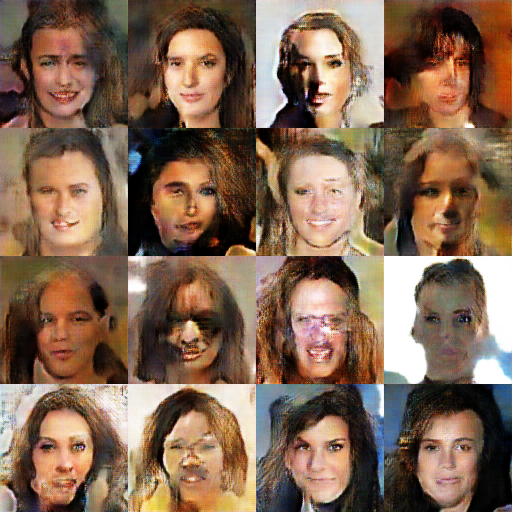
\includegraphics[width=\textwidth]{figures/result_conv_kernel_3.png}
        \caption{Test result using 3×3 convolution kernel after training 4 epochs}
        \label{conv_kernel_3}
    \end{minipage}
\end{figure}


\subsection{Model Overview}

After the research above, we finally obtained the conditional facial image generation and adjustment model.
It is as shown in Figure \ref{smliegan}.

\begin{figure}
    \begin{center}
    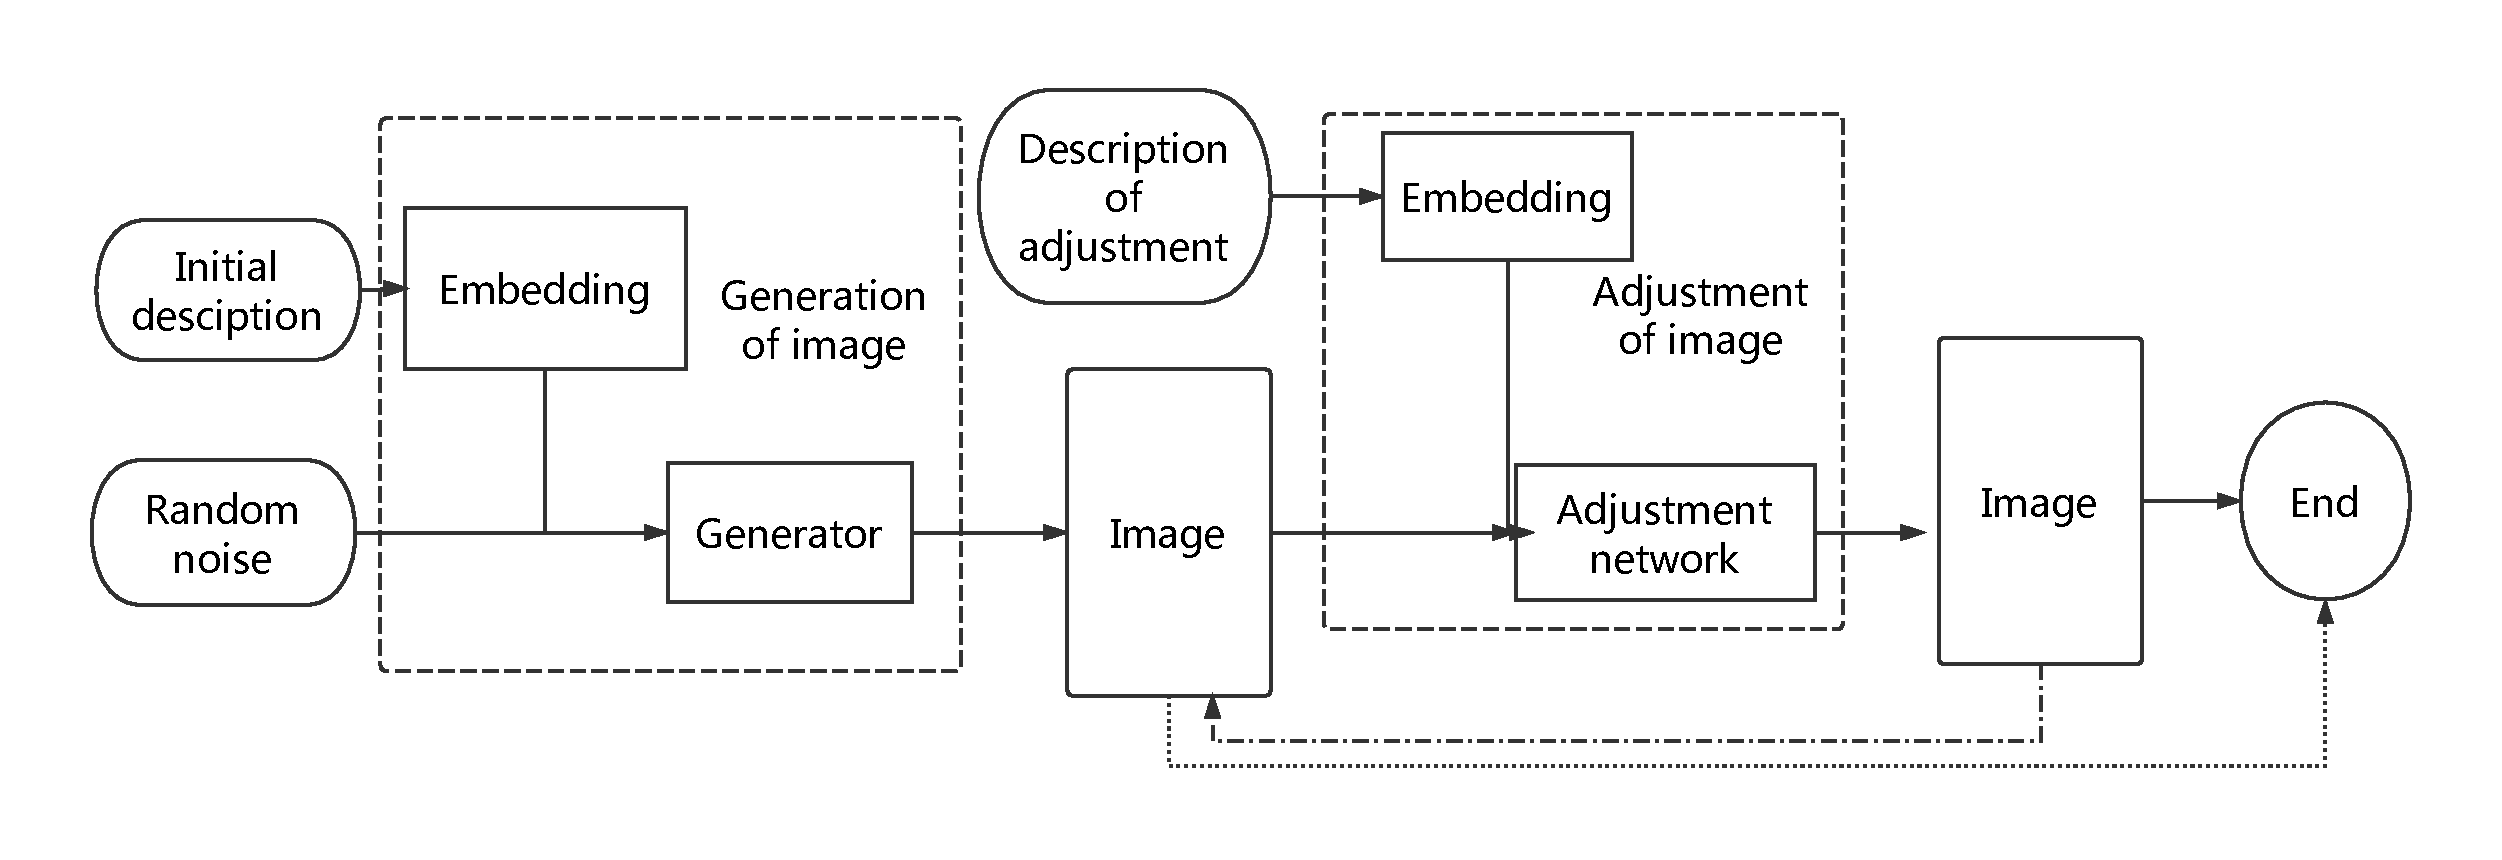
\includegraphics[width=\textwidth]{figures/model.pdf}
    \caption{The Model of LittleGAN}
    \label{smliegan}
    \end{center}
\end{figure}

LittleGAN consists of 3 networks and 2 main components.
The newtworks are generator, discriminator and adjustor.
The main components are encoder and decoder.
In LittleGAN, generator generates facial images from noise and facial attributes,
    and then adjustor combines it with new attributes to obtain new images.


\subsection{Decoder and Encoder}

Main components, encoder and decoder, are used for conversion of feature map and images.

An encoder can extract features from the image from global to local.
Using convolution, starting from an image of 128×128×3 (height × width × channels),
    the convolution with stride is continuously performed.
After each convolution, normalization, activation, dropout\upcite{dropout} is used.

The convolution layer uses a 5×5 convolution kernel.
Convolution filter is 16 in the first layer, doubled in each next layer.
So the image dimension is reduced when the feature is extracted.
    Also, the network has lower calculation amount.
Since we use gradient penalty\upcite{wgan-gp} in training,
    Instance Normalization\upcite{instance} is used at the same time.
To preserve the image for more information, Leaky ReLU (alpha=0.2) is used as the activation function.
In order to prevent occurrence of over-fitting,
    dropout\upcite{dropout} is used in the training to randomly hide some neurons to reduce the interaction between filters.

Decoder is used to generate an image from the feature map.
Using transposition convolution, the same number of filters,
    stride and convolution kernel are symmetrically used with the encoder.
Normalization and activation are performed after each transposition convolution as the same as the encoder.

%todo continue
\subsection{Generator and Discriminator}

We also named the combination of discriminator and generator as GAN network.
Generator consists of a fully connected layer and a decoder.
The facial attributes are combined with latent maps (conform to the normal distribution) as input to generate images by generator.
Discriminator consists of an encoder and 2 fully connected layers.
It uses images as input then extracts features and the probability of image comes from data.


In generator, through a fully connected layer, the input is combined and transformed into feature map(in 4×4×16n size).
Then the image is generated from global to local by decoder layers.
Finally a 3 filters convolution without stride is performed and used.
The tanh function is activated to obtain a three-channel (RGB) color image of 128×128×3 size.
Figure \ref{net_generator} is the graph of generate network structure.

\begin{figure}
    \begin{minipage}[t]{0.48\linewidth}
        \centering
        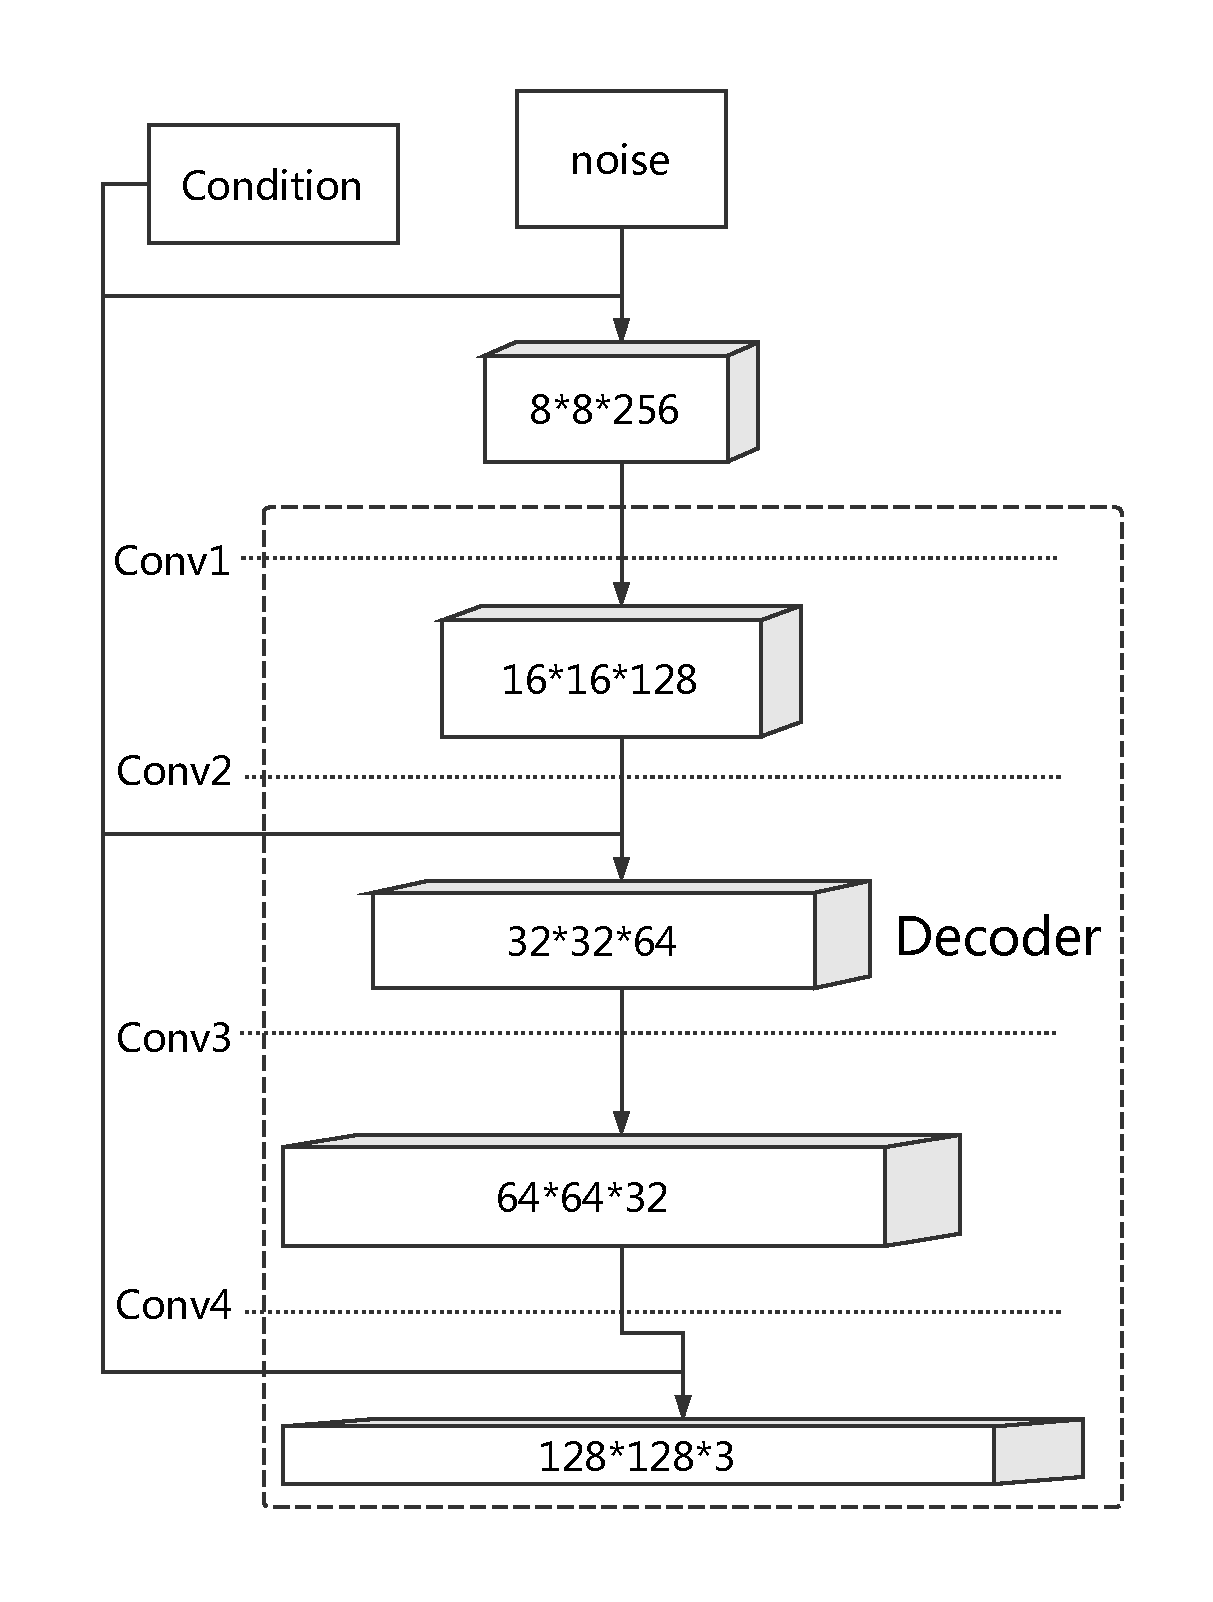
\includegraphics[width=\textwidth]{figures/net_generator.pdf}
        \caption{Generator Network Structure of LittleGAN}
        \label{net_generator}
    \end{minipage}
        \hfill
    \begin{minipage}[t]{0.48\linewidth}
        \centering
        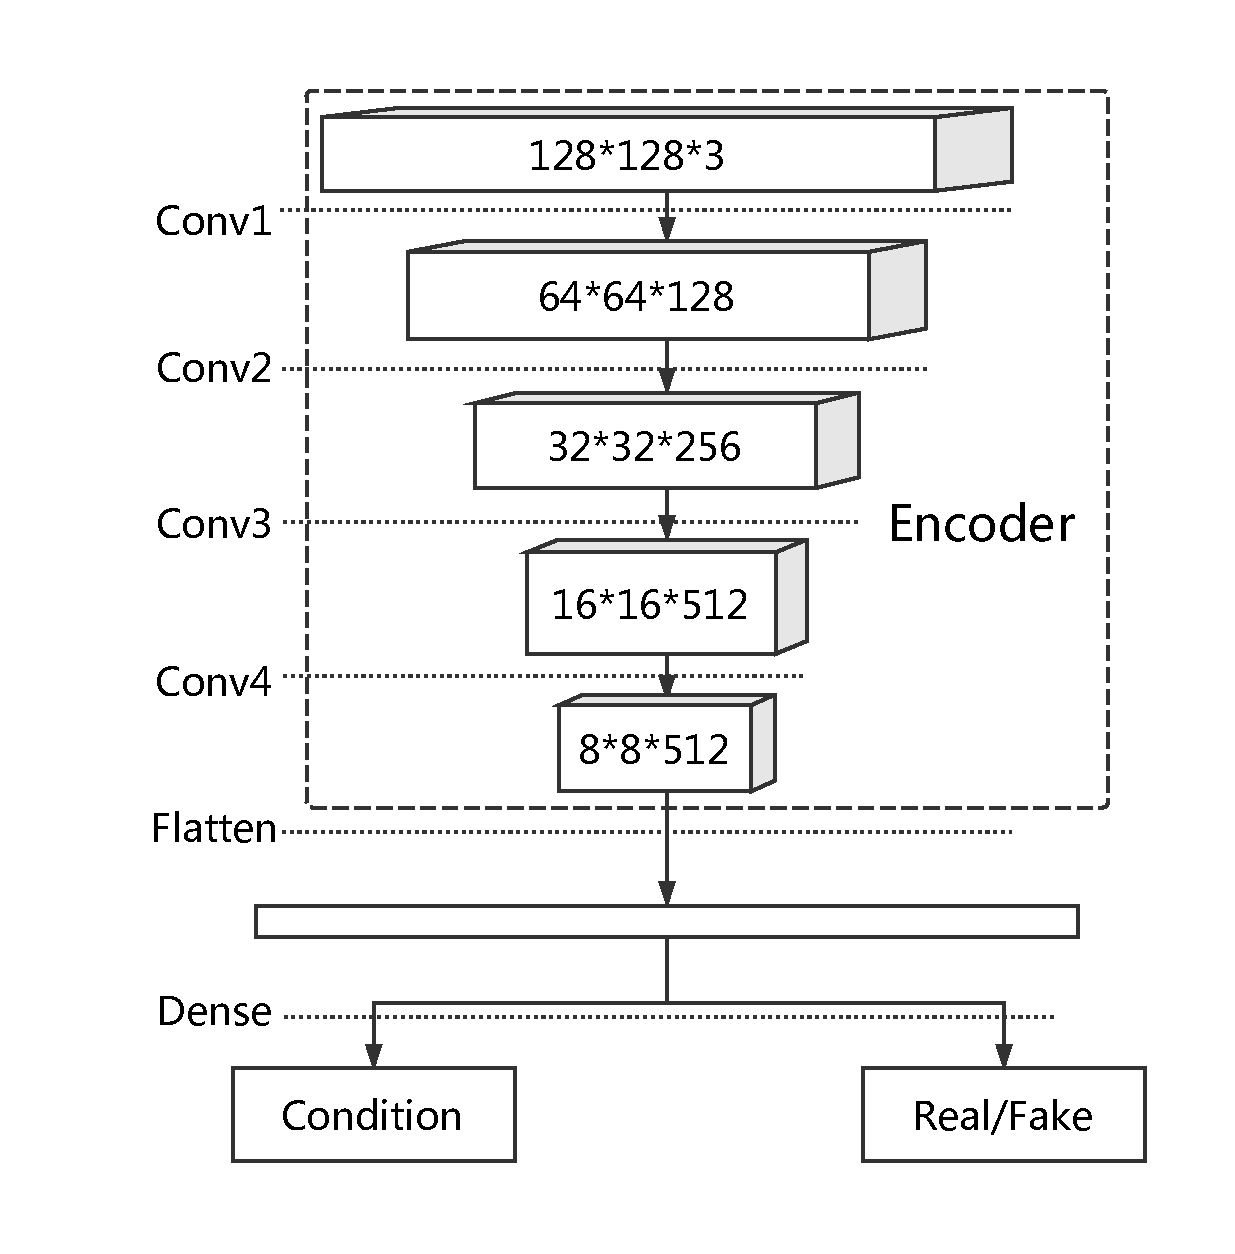
\includegraphics[width=\textwidth]{figures/net_discriminator.pdf}
        \caption{Discriminator Network Structure of LittleGAN}
        \label{net_discriminator}
    \end{minipage}
\end{figure}

Discriminator use encoder to extracts the feature map from the input image first.
Then on the one hand, the feature map is connected to the dimension 1 through a fully connected layer.
The Sigmoid activation function is used to normalize the result to [0,1],
    which indicates the possibility that the image comes from real data.
On the other hand, feature map is connected to the same dimension as attribute,
    the latent facial attribute information is extracted,
    and the result is also normalized to [0,1] using the Sigmoid activation function,
    thereby indicating the possibility that the image has these facial attributes.
Figure \ref{net_discriminator} is the graph of generate network structure.


For discriminator loss function, since the Sigmoid is used to activate the output,
    in order to ensure that the network parameters will not dead,
    we expect the loss of discriminator output to [0.02,0.98] instead of [0,1].
Since discriminator not only outputs probability of image comes from data but also contains the facial attribute information implied by the image,
    its loss includes the GAN loss and the conditional judgment loss.
In discriminator, we expect the output from real image close to 0.98, while the output from fake image close to 0.02.
Similarly, we expect the facial attribute information output by discriminator is as consistent as possible with the real data.
Equation \eqref{loss_d_gan}, Equation \eqref{loss_d_c}, and Equation \eqref{loss_d} are the GAN loss,
    conditional adjustment loss and total loss of discriminator, respectively.

% Todo: Add comment for equation
\begin{equation}
    Loss_{D-GAN}(D,G)=
    \mathbb{E}_{y\thicksim P(data)}[(0.98-D(y))^2]+
    \mathbb{E}_{c,z\thicksim P(fake)}[D(G(c,z)-0.02)^2]
    \label{loss_d_gan}
\end{equation}


\begin{equation}
    Loss_{C}(C)=
    \mathbb{E}_{c,y\thicksim P(data)}[(c-C(y))^2]
    \label{loss_d_c}
\end{equation}

\begin{equation}
    Loss_{D}(C,D,G)=
    Loss_{D-GAN}(D,G)+
    Loss_{C}(C)
    \label{loss_d}
\end{equation}

We add a mean absolute error to generator's loss function.
We expect overall color and layout to be more realistic while keeping the diversity generation results in this way.
The target of generator is to generate an image that treat the discriminator think it's from real data,
    and let discriminator output the attribute close to generation condition.
Therefore, the loss function of generator include into discriminator loss and the mean absolute error loss.
Equation \eqref{loss_g_gan}, Equation \eqref{loss_g_l1}, and Equation \eqref{loss_g} are the discriminator loss,
    mean absolute error loss and total loss of generator, respectively.
The $\lambda$ in the total loss in the experiment is 0.02.

\begin{equation}
    Loss_{G-GAN}(C,D,G)=
    \mathbb{E}_{c,z\thicksim P(fake)}[(0.98-D(G(c,z)))^2]+
    \mathbb{E}_{c,z\thicksim P(fake)}[(c-C(G(c,z)))^2]
    \label{loss_g_gan}
\end{equation}

\begin{equation}
    Loss_{G-L1}(G)=
    \mathbb{E}_{c,y,z\thicksim P(data)}[|y-G(c,z)|]
    \label{loss_g_l1}
\end{equation}

\begin{equation}
    Loss_{G}(C,D,G)=
    Loss_{G-GAN}(C,D,G)+
    \lambda Loss_{G-L1}(G)
    \label{loss_g}
\end{equation}

Our goal is to minimize the loss function of generator and discriminator,
    so the optimization goal of generator against the network is Equation \eqref{gan_target}

\begin{equation}
    GAN^*=\arg \min_{C,D} \max_{G}Loss_{D}(C,D,G)+Loss_{G}(C,D,G)
    \label{gan_target}
\end{equation}


\subsection{Adjustor Network}
Adjustor consists of a decoder, an encoder, several shortcut channels and a combined channel of adjustment conditions.
It uses an encoder to extract features from global to detail,
    and transmits each layer feature to the decoder network through a shortcut channel.
This makes each layer of the network does not need to carry all the information of the image.
Adjuster uses the decoder to combine the extracted features and adjustment conditions step by step to generate an image from detail to global.

Figure \ref{net_adjustor} is the graph of generate network structure.

\begin{figure}
    \begin{center}
    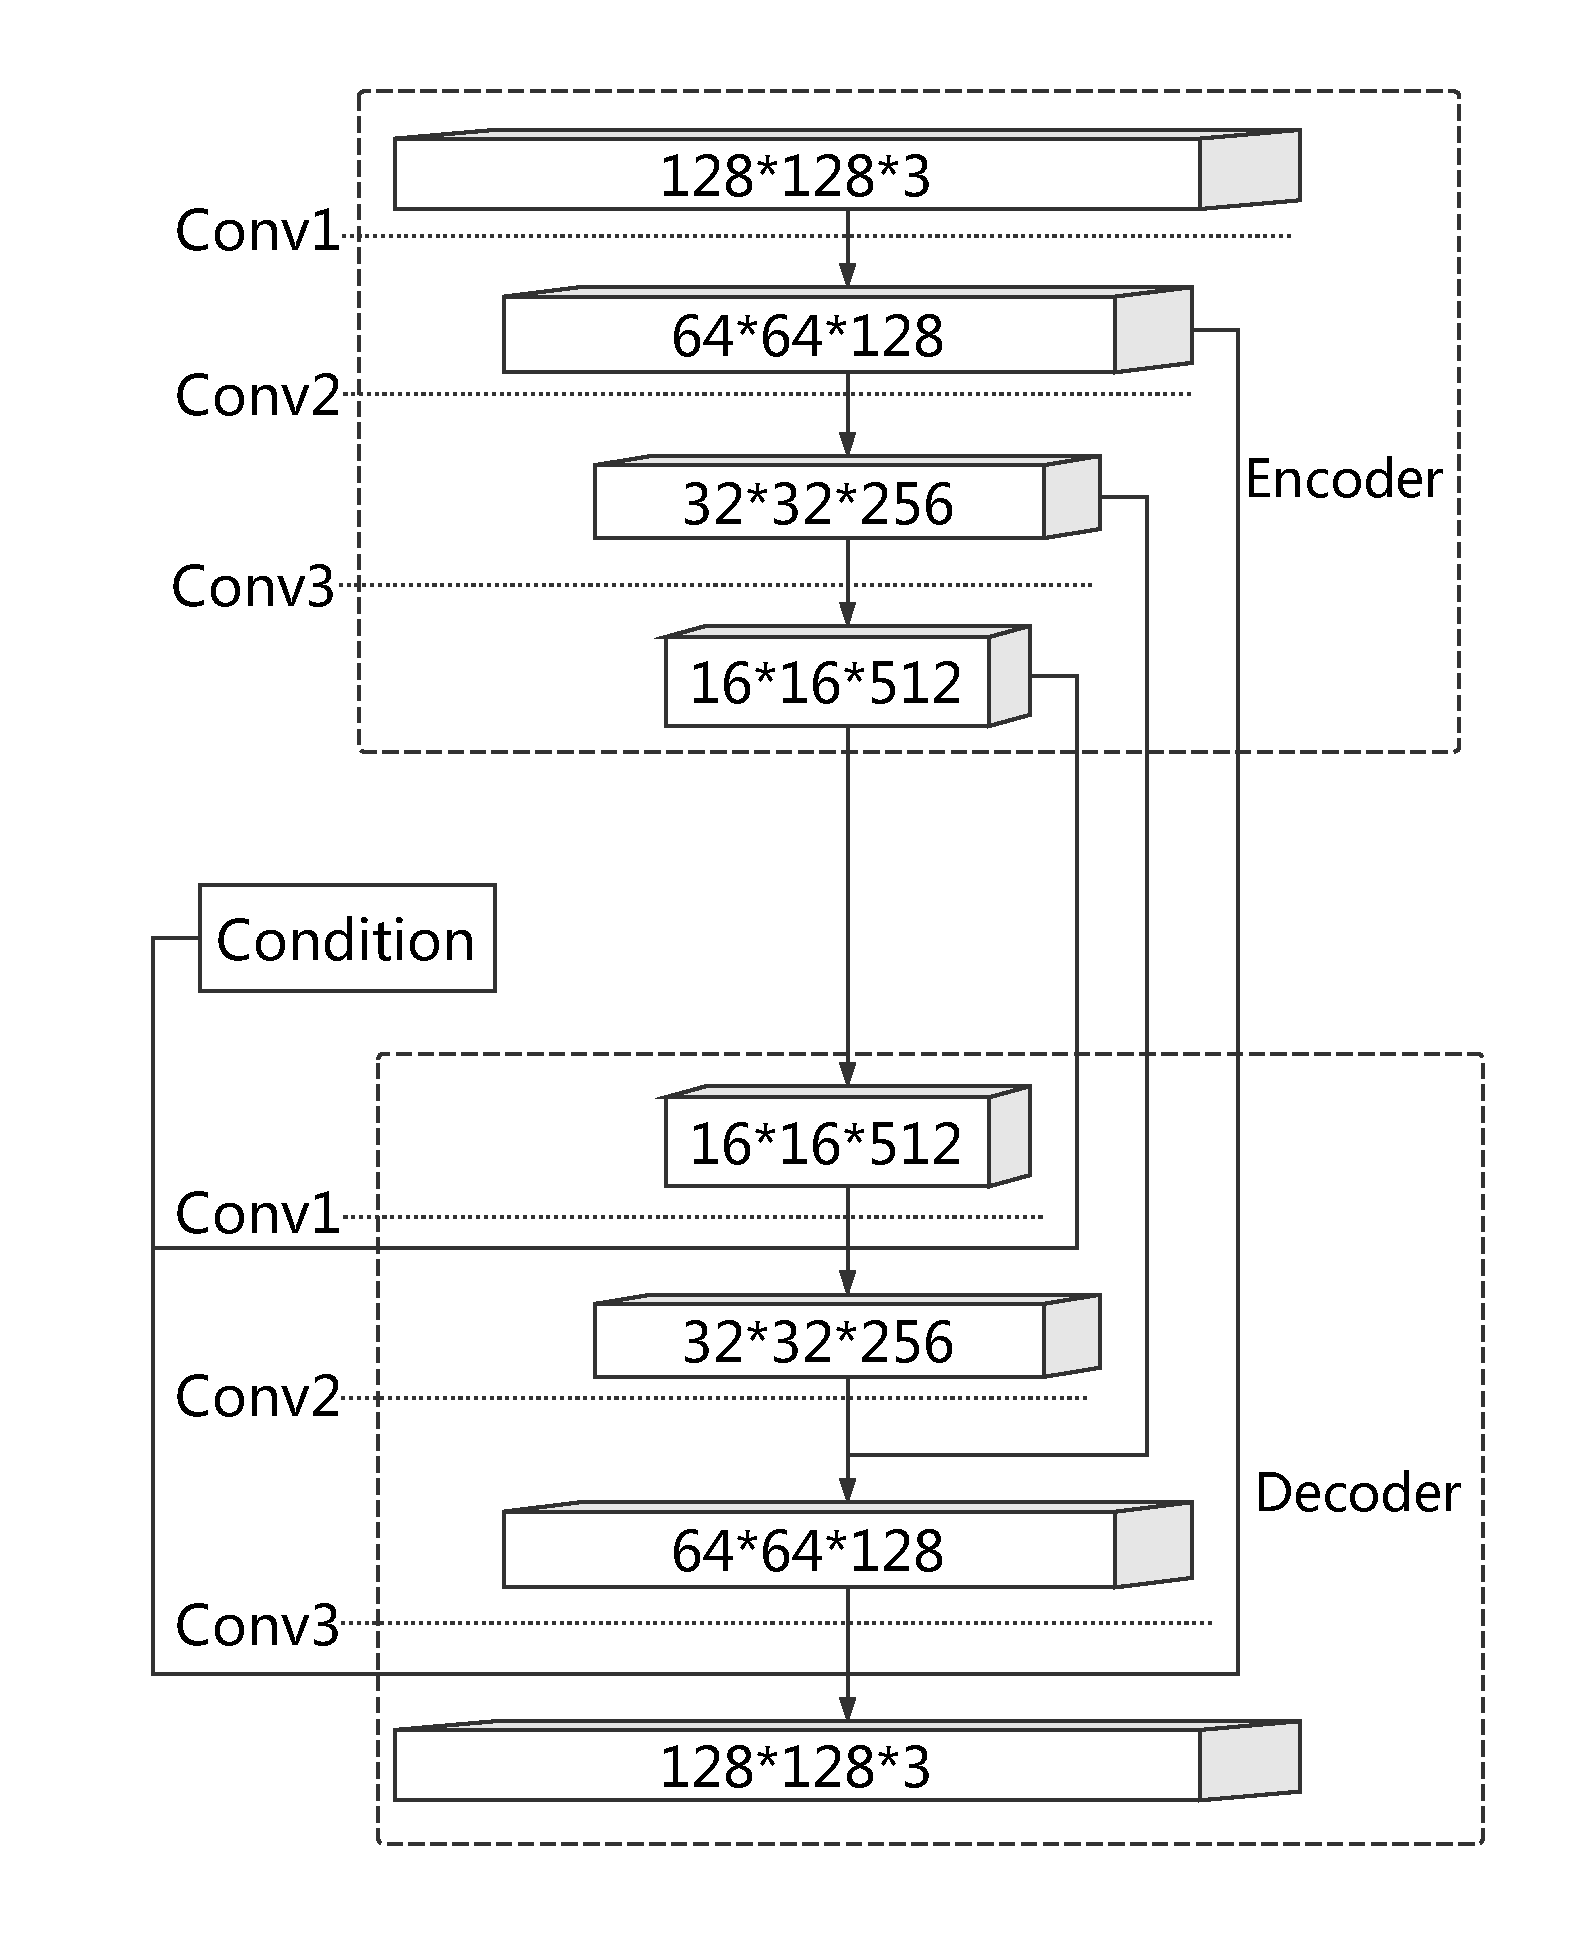
\includegraphics[width=0.48\textwidth]{figures/net_adjustor.pdf}
    \caption{Adjustor Network Structure of LittleGAN}
    \label{net_adjustor}
    \end{center}
\end{figure}

In adjustor network, the decoder and encoder parameters are shared with GAN's.
We use GAN loss and absolute mean error as a loss function for adjustor network.
Equation \eqref{loss_a_gan}, Equation \eqref{loss_a_l1}, and Equation \eqref{loss_u} are the GAN loss,
    mean absolute error loss and total loss of adjustor, respectively.

\begin{equation}
    Loss_{A-GAN}(C,D,A)=
    \mathbb{E}_{c,y\thicksim P(data)}[(0.98-D(A(c,y)))^2]+
    \mathbb{E}_{c,y\thicksim P(data)}[(c-C(A(c,z)))^2]
    \label{loss_a_gan}
\end{equation}

\begin{equation}
    Loss_{A-L1}(A)=
    \mathbb{E}_{c,x,y\thicksim P(data)}[|y-A(c,z)|]
    \label{loss_a_l1}
\end{equation}

\begin{equation}
    Loss_{A}(C,D,A)=
    Loss_{A-GAN}(C,D,A)+
    \lambda Loss_{A-L1}(A)
    \label{loss_u}
\end{equation}

\subsection{Model Training}
There are two main improvements to the training method of the model:
    applying the gradient penalty\upcite{wgan-gp} to discriminator,
    improving the convergence speed and the stability;
    using the partition training that proposed by us,
    enables the network to adjust the previous network layer more effectively,
    so that speed up the convergence.

The specific operation of the partition training proposed by us is as follows.
The network layer parameters that need to be trained in the model are grouped according to the function and the number of parameters.
When training each group of parameters,
    other parameters are fixed and only the parameters in the group are back-propagated.
In practice, for the overall effect of the model,
    we generally cross the overall model training and partition training in a certain proportion.
We set up separate optimizers for each set of parameters if use graph mode.
Although this will take up more memory for the training device,
    it can reduce the CPU's burden that the optimizer frequently switches the optimization target and reconstructs the model.
\section{Experiments}

\subsection{Experiment Environment}
We implement our model using Python 3.6, Tensorflow 1.12 and Keras 2.2.
The model is trained on a single NVIDIA TITAN X (Pascal) GPU in each experiment on Ubuntu 16.04 OS.


\subsection{Dataset}
We use the public dataset CelebA\upcite{celeba}, which contains 202,599 facial images and 40 labelled attributes for each face.
We align and crop the facial images into three-channel(RGB) images of 128×128 pixels and then divide them into training sets, test sets and verification sets according to the ratio of 8:1:1.
For the 40 attributes in the dataset, we select 7 of them: 'gender', 'skin tone', 'hair color', 'beard', 'wear glasses', 'young', 'lipstick' attribute to verify the feasibility of the model.

\subsection{Experimental Items}
\begin{itemize}
\item In order to obtain a suitable model structure and training hyperparameters, we have designed multiple sets of comparative experiments to test the effects of different improvement projects.
\item In order to verify that our model can generate plausible facial images according to input conditions and it has practicability, we have set up experiments of generating and adjusting facial images.
\item To prove our method owns lower use-cost, we have also set up a set of model size comparison experiments.
\end{itemize}

\subsection{Training Details}

We use the Adam\upcite{adam} optimizer to optimize the network.
The learning rates of the discriminator, the generator and the adjustor network are set to $1\times10^{-4}$.
$\beta1$ and $\beta2$ select the default configuration in Adam's\upcite{adam} paper, which is respectively 0.5 and 0.9.
The $\alpha$ in Leaky ReLU\upcite{leaky} is set to $0.3$.
The dropout\upcite{dropout} rate is set to $0.5$.
The encoder network is fixed when training the adjustor network.
The $\lambda$ in both the generator and the adjustor network is set to 0.02.
We use 93-dimensional noise vector and 7-dimensional attributes vector as input.
Use 32 images training set for training.
A total of 20 training sessions are used.
In each batch, the generator is used to generate the image first.
Then the discriminator is used to identify the image and adjusted by the adjustor network.
The calculation results of discriminator are on gradient penalty.
The losses of the discriminator, the generator and the adjustor network are calculated respectively. 
Then the respective optimizers separately performs backpropagation and optimizes network weight parameters.
In the partition training, the overall model training and the partition training are performed in a 4:1 ratio.

\subsection{Evaluation Metric}
It is difficult to evaluate the performance of generative models (e.g., GANs).
In our experiments, we choose the recently proposed metric Fr\'echet Inception Distance\upcite{fid} (FID) to evaluate our experiments.
It considers not only the synthetic data distribution but also how it compares to the real data distribution.
It directly measures the distance between the synthetic data distribution $p(.)$ and the real data distribution $p_r(.)$.
In practice, images are encoded with visual features by the inception model.
Assuming the feature embeddings follow a multidimensional Gaussian distribution,
    the synthetic data's Gaussian with mean and covariance $(m, C)$ is obtained from $p(.)$ and the real data's Gaussian with mean and covariance $(m_r, C_r)$ is obtained from $p_r(.)$.
The difference between the synthetic and real Gaussians is measured by the Fr\'echet distance, \emph{i.e}., $FID = ||m-m_r||_{2}^{2} + Tr\left(C + C_r - 2(CC_r)^{1/2}\right)$. Lower FID values mean closer distances between synthetic and real data distributions.
To compute the FID score for a unconditional model, 30k samples are randomly generated. To compute the FID score for a text-to-image model, all sentences in the corresponding test set are utilized to generate samples. \upcite{stackgan}


\subsection{Experiment Result}
\subsubsection*{More Efficient Generation}


Table \ref{result_speed} shows that the image generation speed of LittleGAN and DCGAN\upcite{dcgan}.
It runs on the computer with an Intel Core i7-6700 CPU.
It shows that the generate speed of LittleGAN is much faster.
It also means that LittleGAN will get higher real-time performance when deployed on computer or mobile devices.

\begin{table}
    \caption{Generate Speed Comparison}
    \label{result_speed}
    \centering 
    
    \begin{threeparttable}
        \begin{tabular}{c|c}
            \hline
            Experiment Name & Time       \\ \hline
            DCGAN        &  11.50s$\pm$0.21s\\
            Final\tnote{*}        &  3.29s$\pm$0.20s\\
            16x-Filter\tnote{*}        & 2.02$\pm$0.14s \\
            Size-5x5\tnote{*}        &  4.85s$\pm$0.07s\\
            48x-Filter\tnote{*}        & 9.91s$\pm$0.25s  \\ \hline
        \end{tabular}

        \begin{tablenotes}
            \item The 200 facial image generation time usage of LittleGAN and DCGAN.
            \item[*] This means the experiment model is LittleGAN.
        \end{tablenotes}
    \end{threeparttable}
\end{table}
Table \ref{result_fid} shows the FID metric of each model.
Lower is better for the metric.
The result of LittleGAN is after training 20 epochs.
Each experiment of LittleGAN takes us about 13.5 hours.
The mode collapse occurs on the whole DCGAN\upcite{dcgan} after training 16 epochs,
    which leads to the failure of the network.
    So, we select the result of DCGAN\upcite{dcgan}after training 15 epochs.
It can be seen that with the improvements,
    LittleGAN gets a better score than DCGAN\upcite{dcgan}.
    It also shows that LittleGAN's performance of generation image is available.
We find some FID\upcite{fid} statistical data on CelebA\upcite{celeba} dataset from the paper "Are GANs Created Equal? A Large-Scale Study"\upcite{gan-compare},
    while their models output the image size of 64x64.
In that case, their metrics will be much bigger at the same condition of ours.

\begin{table}
    \centering
    \caption{FID Metric Comparison}
    \label{result_fid}
    \begin{threeparttable}
    \begin{tabular}{l|ccccc}
        \hline
        Exp. Name    & Kernel Size & Filter Num.   & Partition          & Norm.         & FID            \\ \hline
        Final*        & 3x3         & 24x           & $\surd$            & Instance      & 57.94$\pm$0.09 \\
        Batch*        & 3x3         & 24x           & $\surd$            & Batch         & 59.35$\pm$0.64 \\
        16x-Filter*   & 3x3         & 16x           & $\surd$            & Instance      & 62.82$\pm$0.40 \\
        48x-Filter*   & 3x3         & 48x           & $\surd$            & Instance      & 59.35$\pm$0.42 \\
        Size-5x5*     & 5x5         & 24x           & $\surd$            & Instance      & 56.99$\pm$0.24 \\
        No-Partition* & 3x3         & 24x           & $\times$           & Instance      & 64.22$\pm$0.46 \\ \hline
        DCGAN        & 5x5         & 64x           & $\times$           & Batch         & 77.57$\pm$1.27 \\ \hline
        VAE(64x64)   & -           & -             & $\times$           & -             & 85.7 $\pm$3.8**  \\
        BEGAN(64x64) & 3x3         & 128x          & $\times$           & -             & 38.9 $\pm$0.9**  \\
        WGAN-GP(64x64) & 5x5       & 128x          & $\times$           & Batch         & 30.0 $\pm$1.0**  \\ \lasthline
    \end{tabular}
    
    \footnote{}
    \begin{tablenotes}
        \item The FID metric comparison between serval models.
        \item[*] This means the experiment model is LittleGAN.
        \item[**] this means the FID result is calculated by the paper from Google Brain "Are GANs Created Equal? A Large-Scale Study" 
    \end{tablenotes}
\end{threeparttable}
\end{table}


\subsubsection*{More Stable}
Figure \ref{loss_part_on_d} and \ref{loss_dcgan_d} are the discriminator's loss changes of LittleGAN and DCGAN\upcite{dcgan}.
Figure \ref{loss_part_on_g} and \ref{loss_dcgan_g} are the generator's loss changes of LittleGAN and DCGAN\upcite{dcgan}.
To better measure the convergence speed of LittleGAN and DCGAN\upcite{dcgan},
    we use TensorBoard visualization tool to generate a loss map of the network during training.
By comparison, it can be found that compared with DCGAN\upcite{dcgan},
    the loss of our network changes more smoothly, the variance is smaller and is steadily decreasing.
While DCGAN\upcite{dcgan} often appears to have a fitting and lead to a sudden increase in loss.

\begin{figure}
    \begin{minipage}[t]{0.49\linewidth}
        \centering
        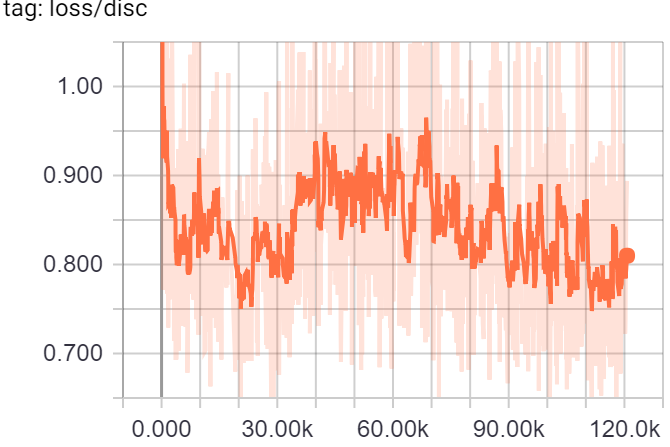
\includegraphics[width=\textwidth]{figures/loss_part_on_d.png}
        \caption{Loss line chart of LittleGAN's Discriminator (turn partition training on)}
        \label{loss_part_on_d}
    \end{minipage}
        \hfill
    \begin{minipage}[t]{0.49\linewidth}
        \centering
        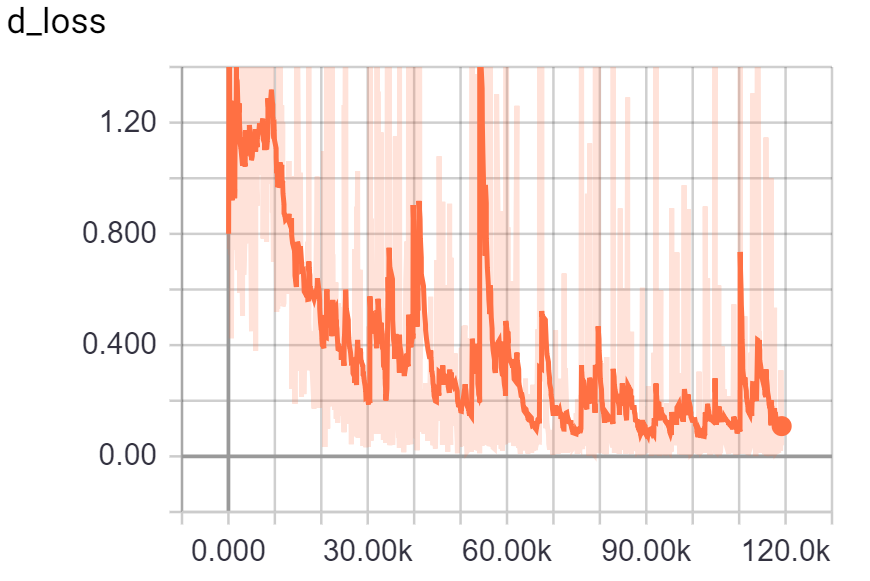
\includegraphics[width=\textwidth]{figures/loss_dcgan_d.png}
        \caption{Loss line chart of DCGAN's Discriminator}
        \label{loss_dcgan_d}
    \end{minipage}
\end{figure}

\begin{figure}
    \begin{minipage}[t]{0.49\linewidth}
        \centering
        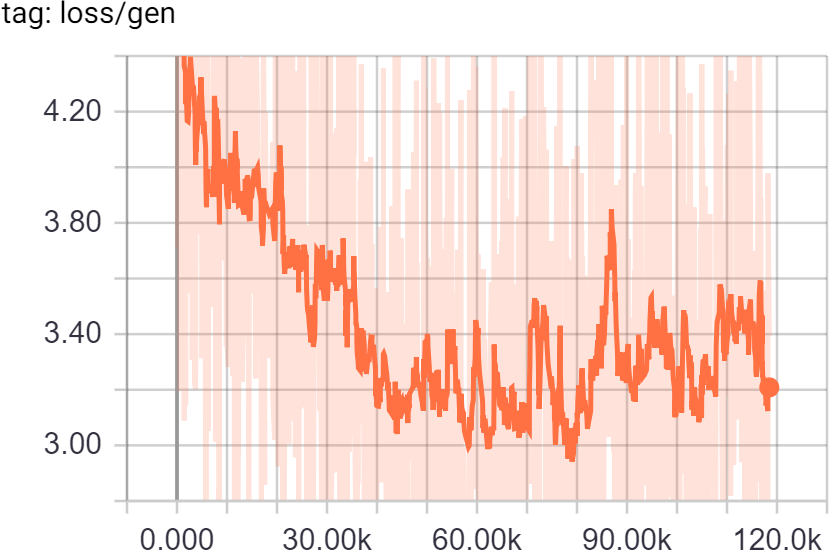
\includegraphics[width=\textwidth]{figures/loss_part_on_g.png}
        \caption{Loss line chart of LittleGAN's Generator (turn partition training on)}
        \label{loss_part_on_g}
    \end{minipage}
        \hfill
    \begin{minipage}[t]{0.49\linewidth}
        \centering
        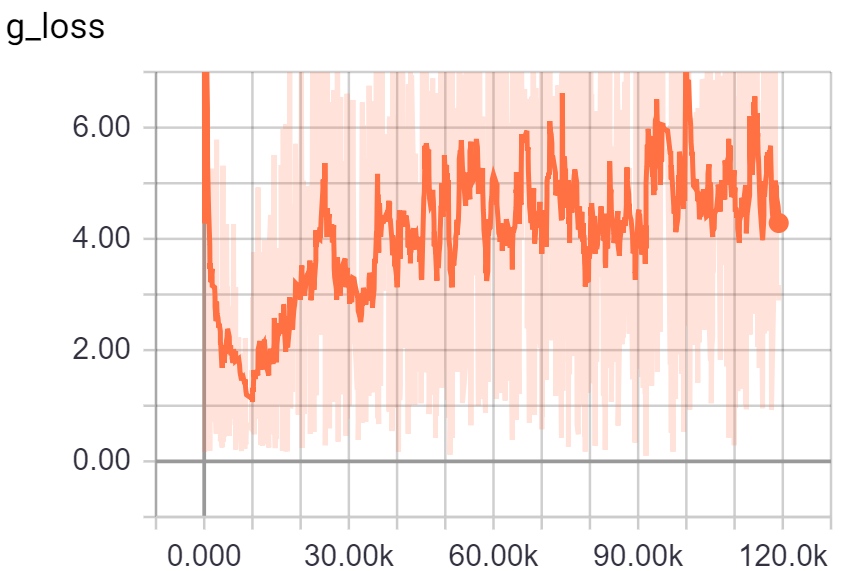
\includegraphics[width=\textwidth]{figures/loss_dcgan_g.png}
        \caption{Loss line chart of DCGAN's Generator}
        \label{loss_dcgan_g}
    \end{minipage}
\end{figure}

Figure \ref{littlegan_e15} and Figure \ref{dcgan_e15} are the test output of LittleGAN and DCGAN\upcite{dcgan} after training 15 epochs of training.
LittleGAN can output very authentic facial images after training 15 epochs.

\begin{figure}
    \begin{minipage}[t]{0.48\linewidth}
        \centering
        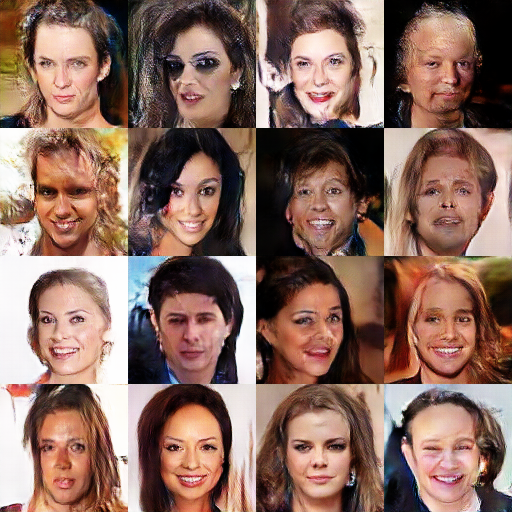
\includegraphics[width=\textwidth]{figures/result_littlegan_e15.png}
        \caption{Test result of LittleGAN after training 15 epochs}
        \label{littlegan_e15}
    \end{minipage}
        \hfill
    \begin{minipage}[t]{0.48\linewidth}
        \centering
        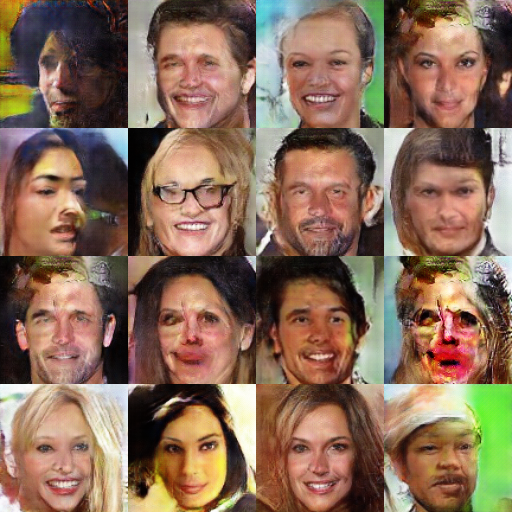
\includegraphics[width=\textwidth]{figures/result_dcgan_e15.png}
        \caption{Test result of DCGAN after training 15 epochs}
        \label{dcgan_e15}
    \end{minipage}
\end{figure}


\subsubsection*{Less Information Loss}
Figure \ref{adjust} is the test result of the generation and adjustment of the facial image.
It can be seen that when the image is roughly consistent, a single feature appears different from other images and other features are not lost.
Our network is able to adjust the specified features of the facial image.

\begin{figure}
    \begin{center}
    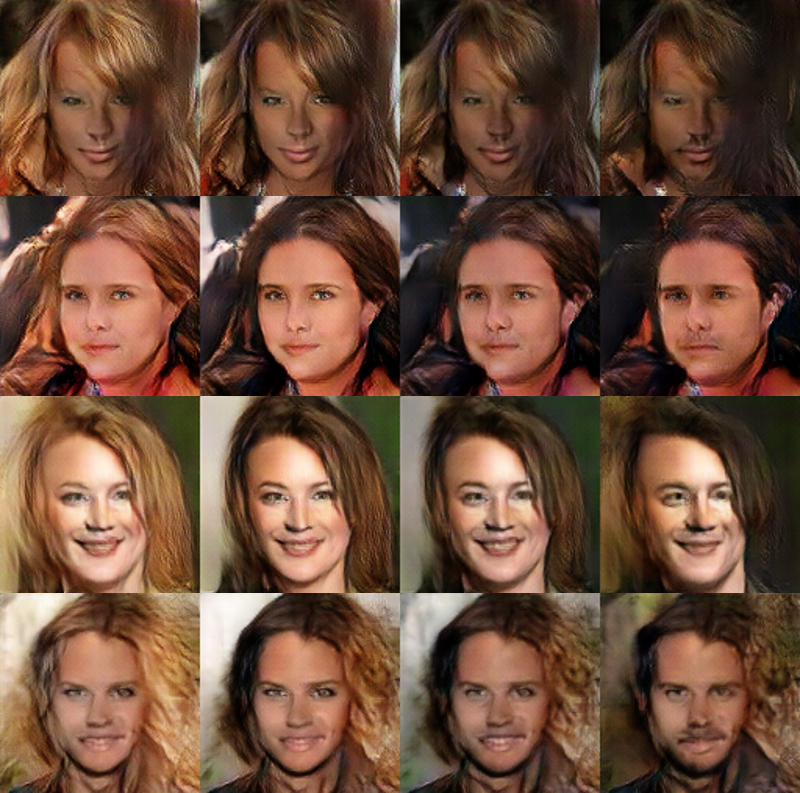
\includegraphics[width=0.49\textwidth]{figures/result_adjust_1.png}
    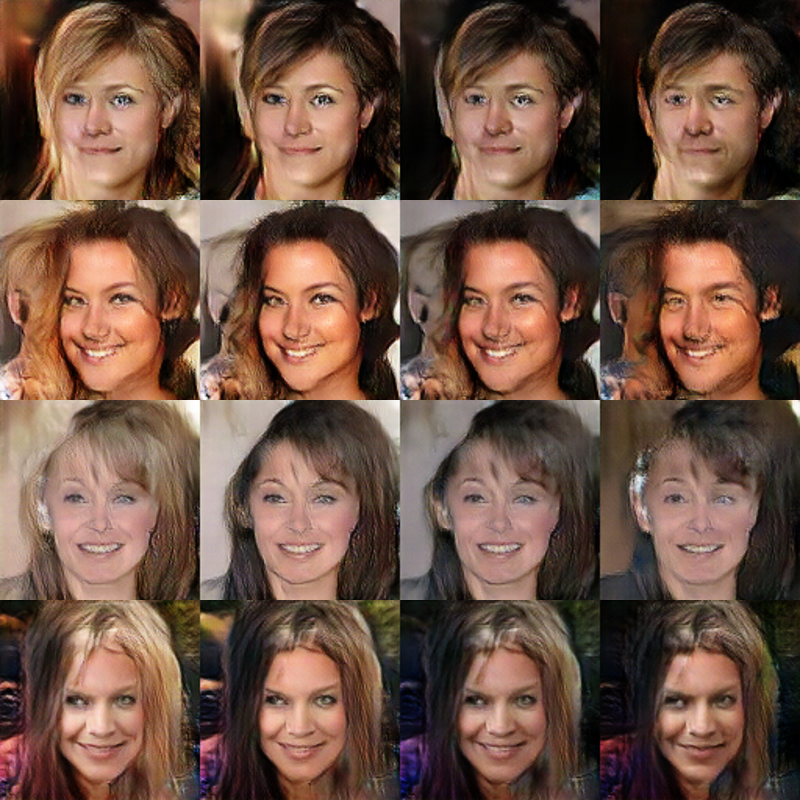
\includegraphics[width=0.49\textwidth]{figures/result_adjust_2.png}
    \caption{Adjustment test result of LittleGAN's Adjustor}
    \label{adjust}
    \end{center}
\end{figure}

\subsubsection*{Faster Convergence}
Figure \ref{littlegan_e1} and Figure \ref{dcgan_e1} show the results after training 1 epoch of training on LittleGAN and DCGAN\upcite{dcgan} on the CelebA\upcite{celeba} training set.
LittleGAN is able to produce clear and highly recognizable facial images after training 1 epoch of training.
Compared to DCGAN\upcite{dcgan}, we can see clearly that the images generated by LittleGAN are sharper and clearer.
It is also closer to the real image in color.
These means that the convergence of LittleGAN is faster than DCGAN at first.

\begin{figure}
    \begin{minipage}[t]{0.48\linewidth}
        \centering
        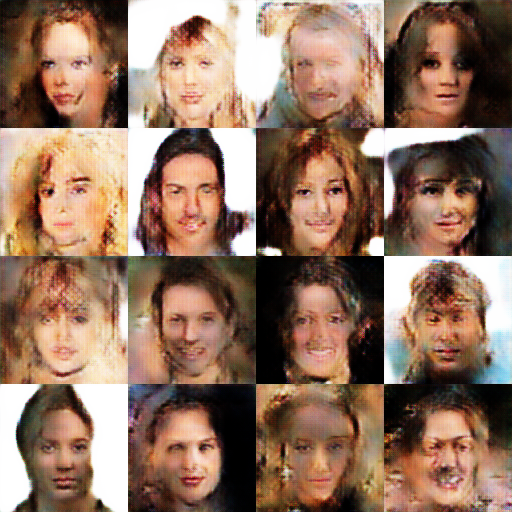
\includegraphics[width=\textwidth]{figures/result_littlegan_e1.png}
        \caption{Test result of LittleGAN after training 1 epoch}
        \label{littlegan_e1}
    \end{minipage}
        \hfill
    \begin{minipage}[t]{0.48\linewidth}
        \centering
        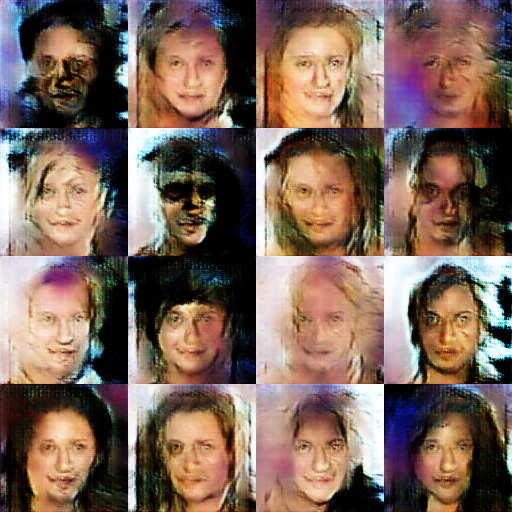
\includegraphics[width=\textwidth]{figures/result_dcgan_e1.png}
        \caption{Test result of DCGAN after training 1 epoch}
        \label{dcgan_e1}
    \end{minipage}
\end{figure}

Fig.\ref{loss_part_on_d}, Fig.\ref{loss_part_on_g}, and Fig.\ref{loss_part_on_u} show the changes of the loss of each components that turn partition training off, respectively.
Fig.\ref{loss_part_off_d}, Fig.\ref{loss_part_off_g}, and Fig.\ref{loss_part_off_u} show the changes of the loss of each components that turn partition training off, respectively.
It can be seen that the loss of the generator reaches the balance faster with partition training started.
 The loss of the discriminator also has a small amplitude and becomes stable.
Figure \ref{part_on} and Figure \ref{part_off} show the test output of the partition training on and off, respectively.
After training 20 epochs, with partition training on, image quality is improved under the same training amount.
These also means that the convergence of LittleGAN is faster than DCGAN at last.

\begin{figure}
    \begin{minipage}[t]{0.48\linewidth}
        \centering
        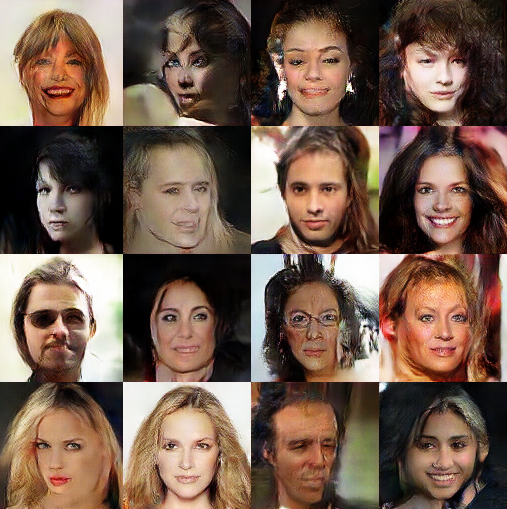
\includegraphics[width=\textwidth]{figures/result_part_on.png}
        \caption{Test result after training 20 epochs (turn partition training on)}
        \label{part_on}
    \end{minipage}
        \hfill
    \begin{minipage}[t]{0.48\linewidth}
        \centering
        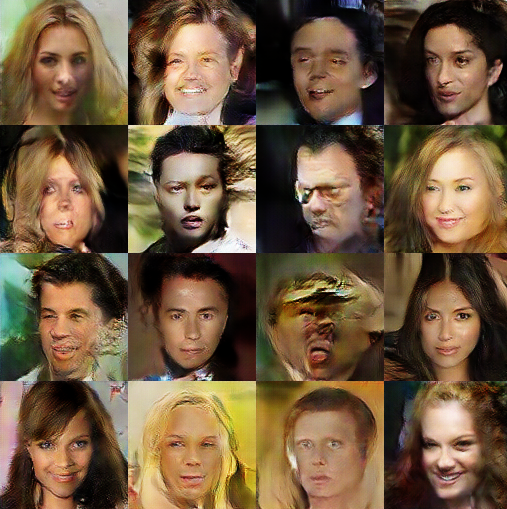
\includegraphics[width=\textwidth]{figures/result_part_off.png}
        \caption{Test result after training 20 epochs (turn partition training off)}
        \label{part_off}
    \end{minipage}
\end{figure}

\begin{figure}
    \begin{minipage}[t]{0.49\linewidth}
        \centering
        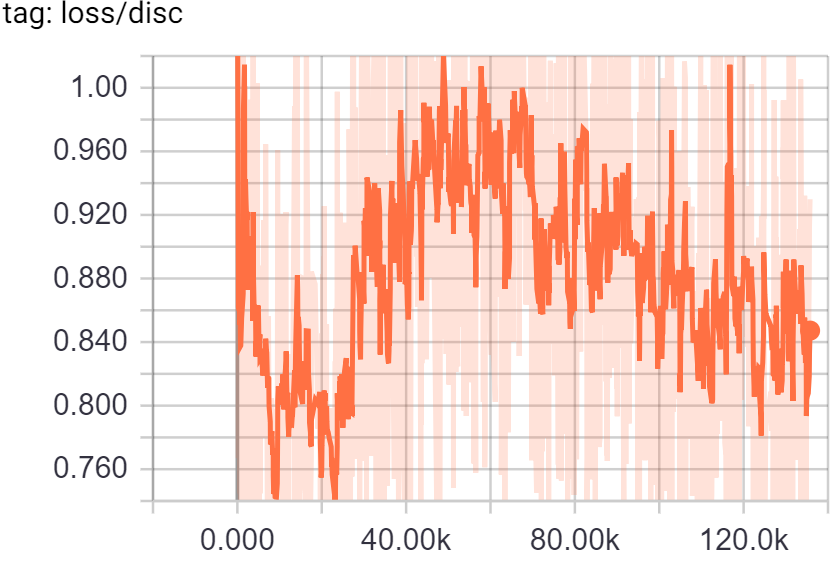
\includegraphics[width=\textwidth]{figures/loss_part_off_d.png}
        \caption{Loss line chart of LittleGAN's Discriminator (turn partition training off)}
        \label{loss_part_off_d}
    \end{minipage}
        \hfill
    \begin{minipage}[t]{0.49\linewidth}
        \centering
        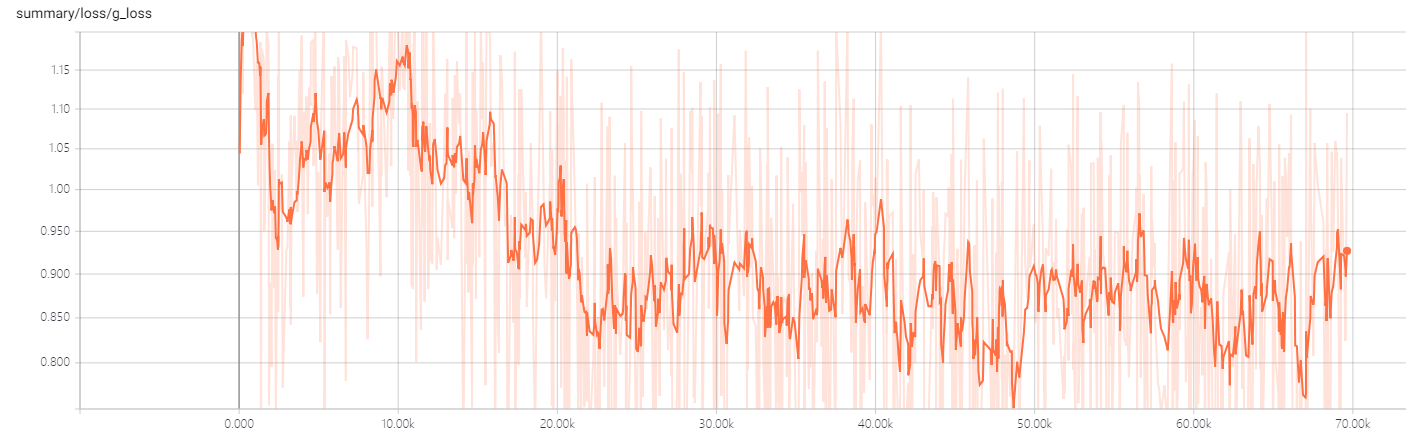
\includegraphics[width=\textwidth]{figures/loss_part_off_g.png}
        \caption{Loss line chart of LittleGAN's Generator (turn partition training off)}
        \label{loss_part_off_g}
    \end{minipage}
\end{figure}

\begin{figure}
    \begin{minipage}[t]{0.49\linewidth}
        \centering
        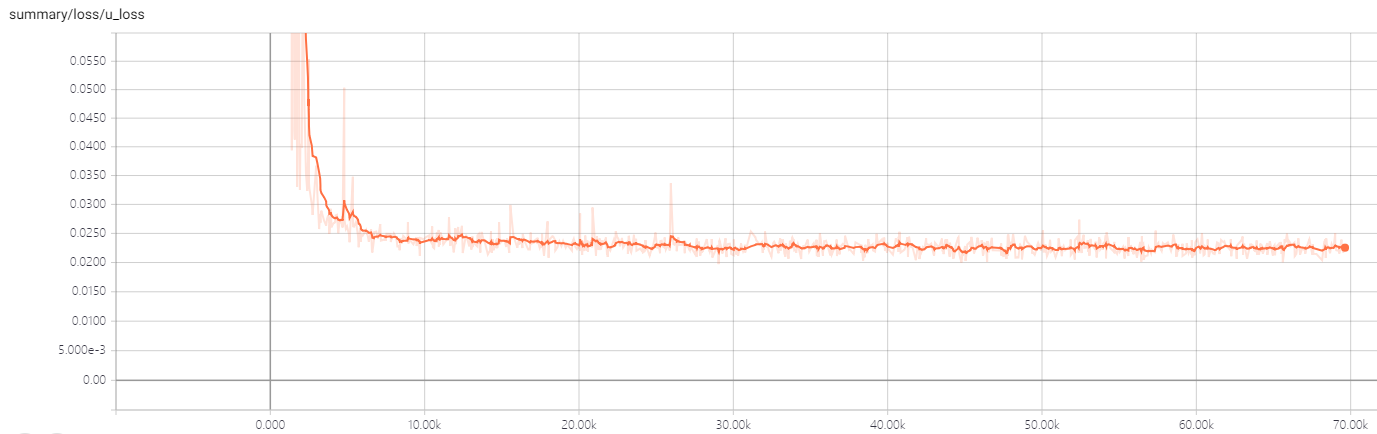
\includegraphics[width=\textwidth]{figures/loss_part_off_u.png}
        \caption{Loss line chart of LittleGAN's Adjustor (turn partition training off)}
        \label{loss_part_off_u}
    \end{minipage}
        \hfill
    \begin{minipage}[t]{0.49\linewidth}
        \centering
        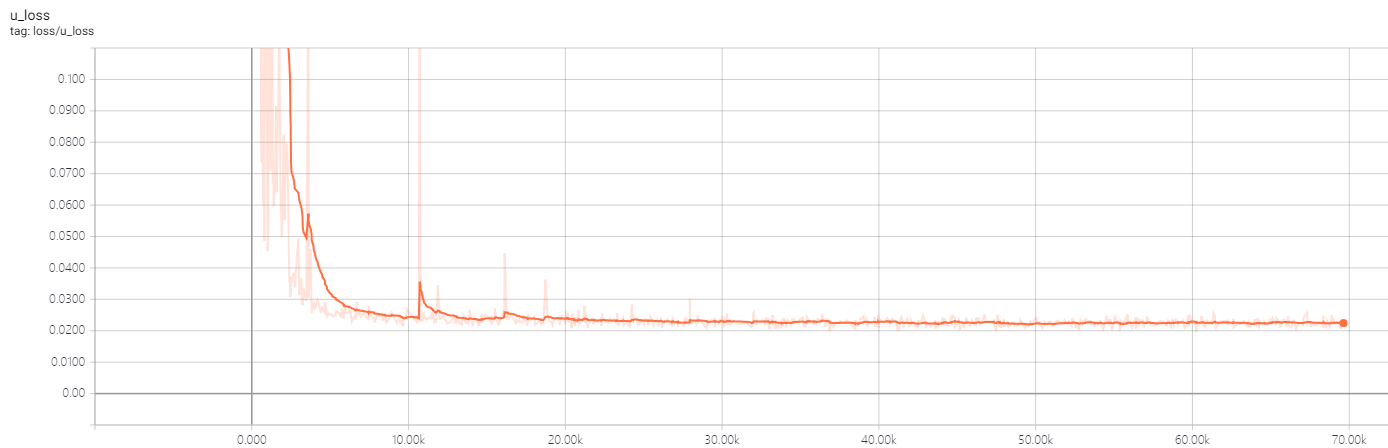
\includegraphics[width=\textwidth]{figures/loss_part_on_u.png}
        \caption{Loss line chart of LittleGAN's Adjustor (turn partition training on)}
        \label{loss_part_on_u}
    \end{minipage}
\end{figure}


\subsubsection*{Lower Use-cost}
We have used a variety of methods to reduce the size of model and the amount of computation.
We compare the model size of pix2pix\upcite{pix2pix}, DCGAN\upcite{dcgan} and LittleGAN when outputting the same size image (a three-channel color image of 128 × 128 pixels).
It is shown in Figure \ref{result_model_size}.
It can be seen that the size of LittleGAN is smaller and LittleGAN costs less.

\begin{figure}
    \begin{center}
    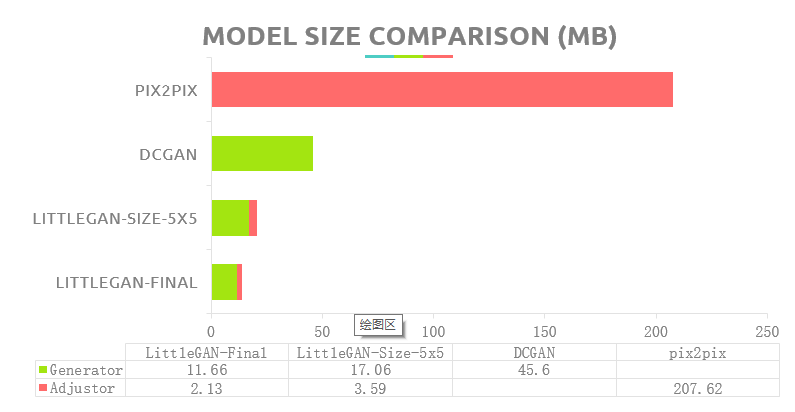
\includegraphics[width=\textwidth]{figures/result_model_size.png}
    \caption{Model Size Comparison}
    \label{result_model_size}
    \end{center}
\end{figure}




\section{Conclusion and Discussion}
\subsection{Conclusion}
In this study, in order to obtain a smaller model with good performance, we have carried out several experiments.
We finally propose a facial image generation and adjustment model and its training method.
We share decoder and encoder among three networks, which are generator, discriminator and adjustor.
In that way, we reduce the model size and the calculation of training.
We adjust facial image in the image space.
It reduces the information loss of original image during the adjustment.
In the training aspect, we use gradient penalty proposed in WGAN-GP\upcite{wgan-gp}.
Most importantly, we creatively put forward partition training.
We have achieved research targets, which are speeding up convergence and further reducing training calculation.

\subsection{Application}
\subsubsection*{Pass portrait information}
In our daily life, in many cases, it is necessary to obtain images of specific person,
    such as conveying the portrait information of strangers and obtaining images in different states.
In the past, general use are verbal descriptions and drawing sketches.
They have poor real-time performance.
Also, requirements for personnel is high.
The information conveyed is not intuitive enough and is easy to be biased.
Our model is small, requires less computing equipment and produces images that are closer to real-world images.
It can be easily deployed in mobile devices to better improve this reality.

\subsubsection*{Expand dataset}
Nowadays, most of machine learning relies on a large amount of data,
    while in reality, there is less data labelled and labelling costs are high.
Using LittleGAN, we can expand dataset.
Machine learning can get more data for training,
    verification and testing.

\subsubsection*{Virtual Character Generation}
On the Internet, for player or non-player characters generation in games,
    individuals or enterprises need personalized avatar generation.
We believe that using this model can meet the above personalized needs at a lower cost.

\subsection{Prospect}

\subsubsection*{More Up-to-date Technologies}

In our pre-study stage, we tried to add a residual layer to the model.
Such an adjustment can make the front network layer of the deep neural network better trained.
But this led to the failure of the model training during the test.
In that case, we eventually abandoned the improvement.
We will next delve into the reasons and apply more new technologies to improve model performance.


\subsubsection*{More Adjustable Attributes}

Due to the lack of some common attributes in the dataset,
    some attributes are not specific enough.
This makes our model's input is not comprehensive enough to generation or adjustment in any way.
Therefore, we will use the method proposed in StarGAN\upcite{stargan},
    which use multiple datasets for training, to enhance the generalization ability of the model.


\subsubsection*{More HD Images}

Due to dataset limitations, the images used for training have lower resolution in our experiments.
Therefore, the image resolution of LittleGAN output is also lower.
In a later improvement, we will try to use a higher resolution labelled facial dataset like CelebA-HQ\upcite{pix2pixhd},
    to train with a higher performance server for a higher resolution model.


\subsubsection*{Natural Language as Input}

Since we did not find suitable natural language description dataset of facial images at first,
    we have canceled the plan to design model with natural language as input.
Next, we will try to create a natural language description dataset of facial images.
The dataset will be used to design and train a model of facial image generation and adjustment with natural language input,
    further reducing the requirements of LittleGAN for users.
Make it easier for users to generate images.


\subsubsection*{Multi-domain Migration}

LittleGAN is to provide a solution to the needs of facial image generation and adjustment.
It is more suitable for production environment.
The improved method we proposed in the study, like partition training, can also be applied to more fields.
We hope to transfer and apply the results and experience gained in our research to more areas and reduce use-cost of training, deployment and running.


\vspace{4ex}

We have open sourced code of our model, training and testing on Github, \url{https://github.com/ixarea/littlegan}.
We are and will continue to conduct in-depth research to further improve and perfect LittleGAN,
    such as improving the performance, expanding the applicable field and improving the ecosystem.
We believe that with our efforts and the help of the community,
    this research project will enter people's production and life.
In that case, everyone can have a more convenient life.








\newpage
\bibliography{references}{}
\bibliographystyle{IEEEtran}

\section*{Acknowledgement}
\addcontentsline{toc}{section}{Acknowledgement}

Meng Yongxiang
Chen Wenyan

Liang Jingyun

Zheng Weishi



\includepdf[noautoscale]{attach/declaration.pdf}
\end{document}

